\chapter{JavaWeb~项目}

\section{设计}
\subsection{前端}
饿了么的前端设计主要采用Vue.js框架进行开发。

\section{测试}
在本项目中,我们先对点餐的正常流程进行了测试,
\begin{enumerate}
\item{注册}:

\begin{itemize}
\item{输入数据}:手机号码:12345678911;密码:123;确认密码:111;用户名称:user;性别:女;
\item {预期结果}:两次输入的密码不一致!
\item {实际结果}:
\begin{figure}[htbp]
\centering
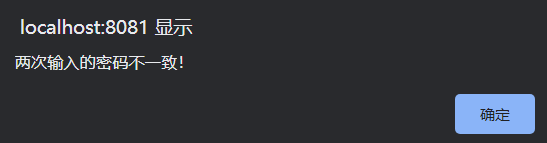
\includegraphics[width=0.6\textwidth]{conflictingPass}
\caption{注册密码不一致图}\label{fig:conflictingPass}
\end{figure}

\item{输入数据}:手机号码:12345678911;密码:123;确认密码:123;用户名称:user;性别:女;
\item {预期结果}:注册成功并跳转至登录页面
\item {实际结果}:注册成功并跳转至登录页面
\begin{figure}[htbp]
\centering
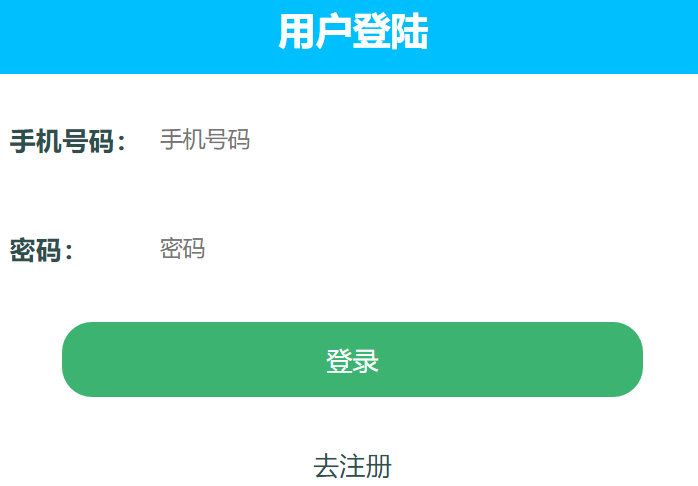
\includegraphics[width=0.6\textwidth]{login1}
\caption{注册成功返回登录的图}\label{fig:login1}
\end{figure}

\item{预置条件}:手机号12345678911已注册
\item{输入数据}:手机号码:12345678911;密码:123;确认密码:123;用户名称:user;性别:女;
\item {预期结果}:此手机号码已存在!
\item {实际结果}:
\begin{figure}[htbp]
\centering
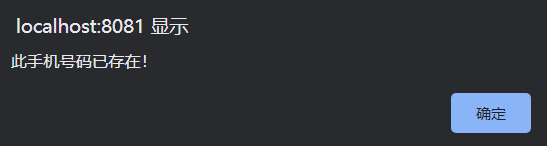
\includegraphics[width=0.6\textwidth]{existingTel}
\caption{重复注册图}\label{fig:existingTel}
\end{figure}
\end{itemize}
\item {登录}:
\begin{itemize}
\item{预置条件}:手机号12345678911已注册
\item{输入数据}:手机号码:12345678911;密码:123;
\item{预期结果}:若上一个页面为注册页面,则返回首页,否则返回登录前的页面
\item{实际结果}:当上一个页面为注册页面时,登录后仍返回注册页面
\item{解决办法}:前端页面跳转至login前,记录来时的路由,并判断是否为register,若是,则登录成功后跳转至首页,否则跳转至来时的路由。
\end{itemize}
\begin{figure}[htbp]
\centering
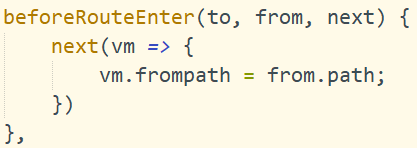
\includegraphics[width=0.4\textwidth]{beforeRouter}
\caption{记录来时的路由}\label{fig:beforeRouter}
\end{figure}
\begin{figure}[htbp]
\centering
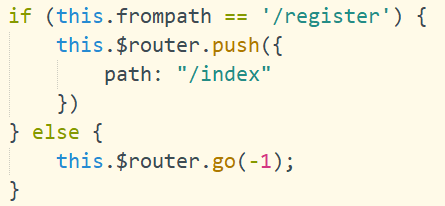
\includegraphics[width=0.4\textwidth]{isRegister}
\caption{判断来时的路由}\label{fig:isRegister}
\end{figure}
\item {“订单”页面}:
\begin{itemize}
\item{操作说明}:点击下拉按钮查看订单详情,点击“去支付”支付订单
\item {预期结果}:可以看到点餐详情,“去支付”后跳转至支付页面
\item {实际结果}:
\begin{figure}[htbp]
\centering
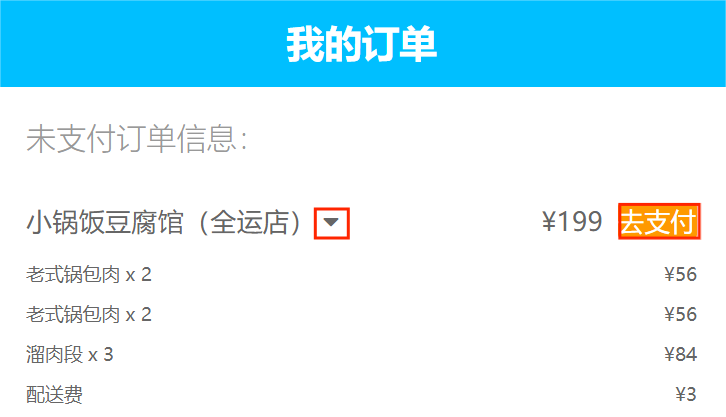
\includegraphics[width=0.4\textwidth]{detail}
\caption{订单详情}\label{fig:detail}
\end{figure}
% \begin{figure}[htbp]
%     \centering
%     \includegraphics[width=0.4\textwidth]{toPay}
%     \caption{去支付}\label{fig:toPay}
% \end{figure}
\end{itemize}

\item {“我的”页面}:
\begin{itemize}
\item{操作说明}:点击用户名旁的编辑按钮,更改用户名为“张三”
\item {预期结果}:“我的”页面用户名更改为“张三”
\item {实际结果}:数据库用户名更改成功,但“我的”页面用户名仍为原用户名
\item {解决办法}:向sessionStorage中存储新的user对象
\begin{figure}[htbp]
\centering
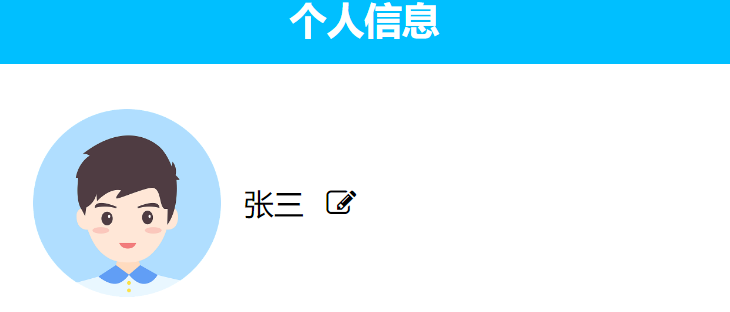
\includegraphics[width=0.6\textwidth]{updateName}
\caption{更改用户名成功图}\label{fig:updateName}
\end{figure}
\item{操作说明}:点击“修改密码”,第一次在“旧密码”中输入错误密码;第二次在“旧密码”中输入正确密码。
\item {预期结果}:第一次修改密码失败;第二次修改密码成功。
\item {实际结果}:第一次修改密码失败;第二次修改密码成功。
\begin{figure}[htbp]
\centering
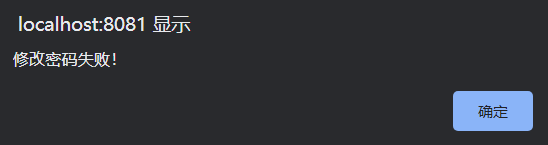
\includegraphics[width=0.4\textwidth]{errorPass}
\caption{更改密码失败图}\label{fig:errorPass}
\end{figure}
\begin{figure}[htbp]
\centering
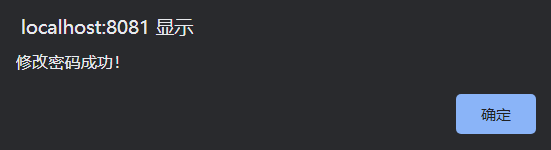
\includegraphics[width=0.4\textwidth]{correctPass}
\caption{更改密码成功图}\label{fig:correctPass}
\end{figure}
\item{操作说明}:点击“我的地址”
\item {预期结果}:进入“地址管理”页面,可进行地址的增删改
\item {实际结果}:完成“地址管理”页面中地址的增删改功能
\begin{figure}[htbp]
\centering
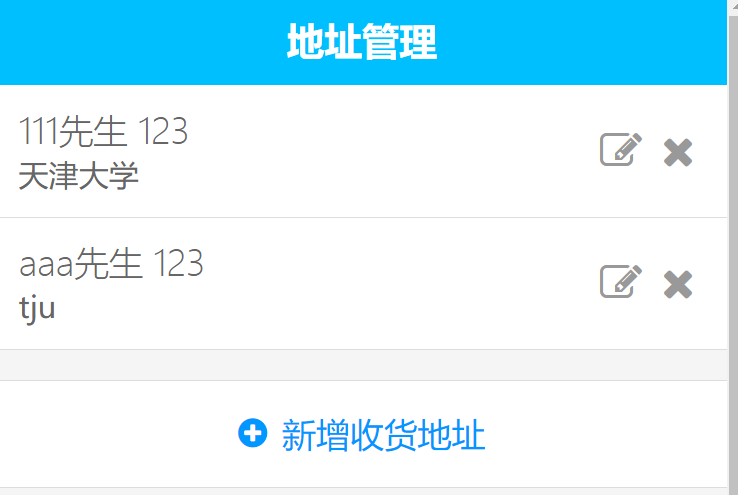
\includegraphics[width=0.4\textwidth]{address}
\caption{地址管理}\label{fig:address}
\end{figure}
\item{操作说明}:点击“退出登录”
\item {预期结果}:返回登录页面,用户再次访问时需登录认证
\item {实际结果}:返回登录页面,但用户再次访问时仍保持登录状态
\item {解决办法}:在退出登录后,前端需要从sessionStorage中移除user对象
\end{itemize}
\begin{figure}[htbp]
\centering
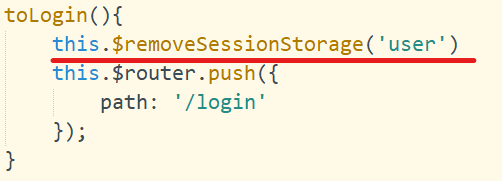
\includegraphics[width=0.4\textwidth]{withdrew}
\caption{退出登录}\label{fig:withdrew}
\end{figure}
\end{enumerate}

\section{部署}
\begin{itemize}
\item{输入数据}:
\item {预期结果}:
\item {实际结果}:
\end{itemize}

